\section{Punto de Vista de Motivación}
En esta vista de motivación permite diseñar al modelador los elementos de motivación por medio de influenciadores. En esta vista se resume las vistas anteriores dando lugar a tener las caracterizaras mas importantes de la vista motivacional.

\subsection{Modelo de Motivación}
\begin{figure}[h!]
	\centering
	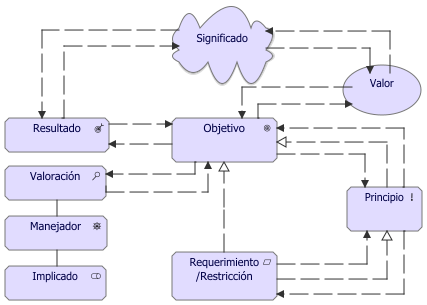
\includegraphics[width=1.0\linewidth]{imgs/modelo/Motivacion}
	\caption{Modelo Motivación}
\end{figure}

Los elementos de motivación se utilizan para modelar las motivaciones, o razones, que guían el diseño o cambio de una arquitectura empresarial. Entre los elementos mas importantes se tiene el implicado: aquel que se implica en el objetivo estudiado, por otro lado tenemos el alcance: aquel que da la motivación, entre otros mas elementos que radican en la motivación e influencia que ejercen sobre los objetivos estratégicos

\clearpage
\subsection{Caso  de Motivación}

\begin{figure}[h!]
	\centering
	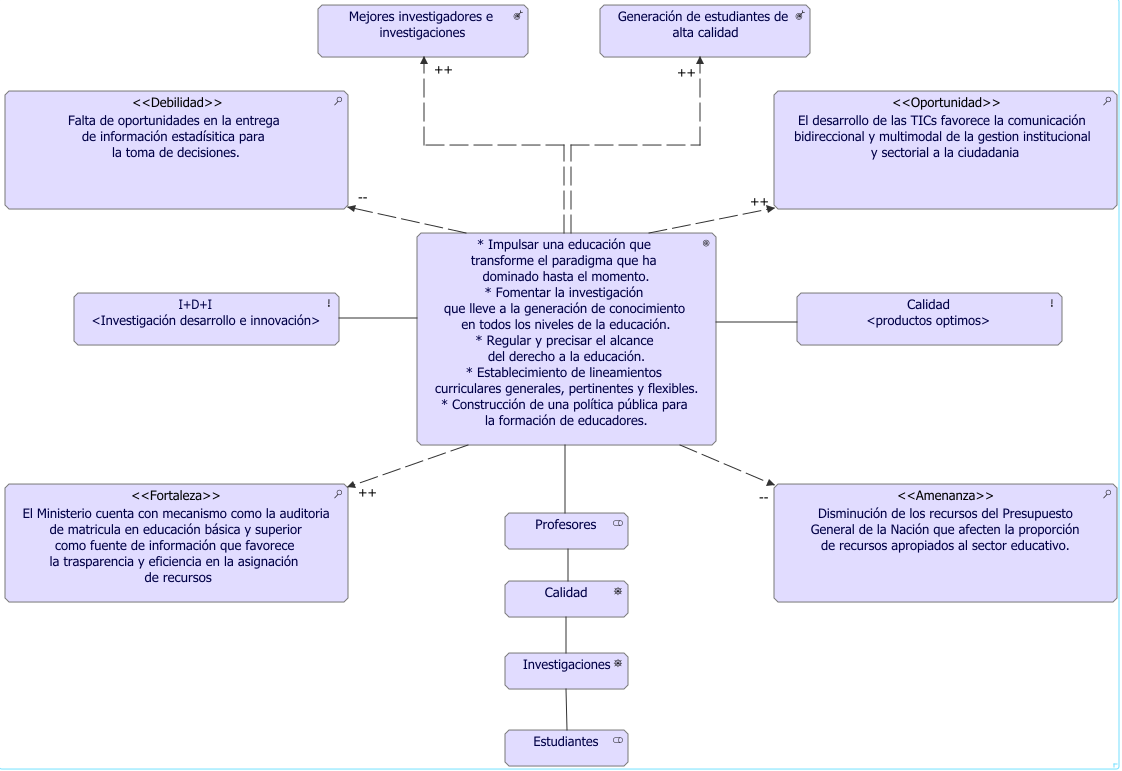
\includegraphics[width=1.0\linewidth]{imgs/motivacion/motivacion/motivacion}
	\caption{Caso Motivación}
\end{figure}

El análisis DOFA es un importante elemento que permite encontrar las estrategias que envuelven objetivos con el fin de mejorar los fines de una empresa. Para los objetivos agrupados en el caso de estudio de motivación tenemos las fortaleza: el ministerio usa la auditoria de la educación para favorecer la eficiencia de los recursos suministrados. La falta de oportunidad para tomar decisiones es una debilidad de la organización. Los implicados que están relacionados con una educación de calidad en este caso de estudio se tienen a los profesores impulsando calidad en sus enseñanzas logrando investigaciones y estudiantes de tal grado.    
